\documentclass{report}

\usepackage[utf8]{inputenc} % For encoding
\usepackage[spanish]{babel}
\usepackage{
	graphicx, % For images
	amsmath, % For math
	geometry, % For page margins
	algorithm,
	algpseudocode,
	hyperref, % For links
}

\graphicspath{{images/}}
\geometry{
	left=1.5cm,
	right=1.5cm,
	top=1.5cm,
	bottom=1.5cm
}
\pagestyle{plain} % Chapter/section in header
\title{
	
\includegraphics[width=0.25\textwidth]{UV.png} \\[1cm]
	Moderando el conflicto interno de opiniones en una red social
}
\author{
	Calderón Prieto Brandon (2125974) \and
	Cely Archila Juleipssy Daianne (2122036) \and
	Fonseca Idarraga Juan David (2323942) \and
	Alvarez Valderrama Jorge Enrique (2125356)
}
\date{\today}


\begin{document}

\maketitle

\pagenumbering{gobble}

\tableofcontents

\clearpage

\pagenumbering{arabic}


\section{Modelo genérico}

\subsection{Parámetros}

\begin{itemize}
	\item $n \in \mathbb{ N }$: número total de personas.

	\item $m \in \mathbb{ N }$: número total de opiniones.

	\item $p \in \mathbb{ N }^m$: vector con la distribución de personas por opinión, donde $p_i$ es el número de personas que inicialmente tienen la opinión $i \in 1\dots m$, $\sum_{ i = 1 }^m p_i = n$.

	\item $e \in [0,1]^m$: vector con los valores de extremismo de las opiniones, donde $e_i \in [0,1]$ es el valor de extremismo de la opinión $i \in 1 \dots m$.

	\item $c$: matriz de costes, donde $c_{ i,j } \in \mathbb{ R }^+$ es el coste de mover una persona de la opinión $i$ a la opinión $j$, para $i,j \in 1 \dots m$ ($c_{ i,i } = 0$).

	\item $ce$: vector de coste extra, donde $ce_i \in \mathbb{ R }^+$ es el coste adicional de mover una persona a la opinión $i$ si esa opinión estaba inicialmente vacía, para $i \in 1 \dots m$.

	\item $ct \in \mathbb{ R }^+$: coste total permitido.

	\item $M \in \mathbb{ N }$: número máximo de movimientos permitidos.
\end{itemize}

\subsection{Variables}

Una matriz $s$, donde $s_{ i,j } \in \mathbb{ N }$ es el número de personas movidas de la opinión $i$ a la opinión $j$, para $i,j \in 1 \dots m$.

Esta matriz es de dimensiones $m \times m$ y debe cumplir las siguientes restricciones:

\begin{itemize}
	\item $\sum_{ j = 1 }^m s_{ i,j } = p_i$: para cada opinión inicial $i$, la suma de personas que se mueven desde esa opinión hacia todas las demás (incluida ella misma) debe ser igual al número de personas que originalmente tenían la opinión $i$. $\sum_{ i = 1 }^m \sum_{ j = 1 }^m s_{ i,j } = n$.

	\item $s_{ i,j } \geq 0$ para todo $i,j \in 1 \dots m$.
\end{itemize}

\subsection{Restricciones}

\subsubsection{Numero de movimientos}

\begin{equation}
	\sum_{ i = 1 }^m \sum_{ j = 1 }^m s_{ i,j } \cdot \abs{ j - i } \leq M
\end{equation}

\subsubsection{Coste total}

\begin{equation}
	\sum_{ i = 1 }^m \sum_{ j = 1 }^m c_{ i,j } \left (1 + \frac{ p_i }{ n } \right ) * s_{ i,j } + \delta_{ p_j, 0 } \cdot ce_j * s_{ i,j } \leq ct
\end{equation}

$\delta_{ p_j, 0 }$ es una función indicadora que vale 1 si $p_j = 0$ y 0 en caso contrario.

\subsection{Función objetivo}

La idea es minimizar el extremismo, que se calcula con la siguiente fórmula:

\begin{equation}
	E(p^\prime,e) = \sum_{ i = 1 }^m { p^\prime }_i * e_i
\end{equation}

- $p^\prime$: vector con la distribución de personas tras aplicar los movimientos de $s$. $p^\prime[j] = \sum_{ i = 1 }^m s[i,j]$ $\forall j = 1\dots m$.

- $e$: vector con los valores de extremismo de las opiniones.

\subsection{Clasificación}

Aunque todas las variables de decisión son enteras, para modelar las restricciones es necesario usar variables de tipo \texttt{float}. Esto hace que el modelo sea un \emph{Programación Lineal Entera Mixta}.

\section{Implementación}

Gracias a las instrucciones de modelado de MiniZinc y la naturaleza del problema, las restricciones y la función objetivo se pueden expresar en pocas líneas de código.

La implementación puede describirse en los siguientes pasos:

\begin{itemize}
	\item Computación de distancias: para evitar el cálculo repetido de las distancias entre opiniones, se crea una matriz $d$ donde $d_{ i,j } = \abs{ i - j }$.

	\item Conservación de flujos ($\sum_{ j = 1 }^m s_{ i,j } = p_i$): se hace con el fin de que nadie "desaparezca". También se añade la restricción $s_{ i,j } \leq p_i$ para acotar dominios y acelerar la búsqueda.

	\item Cálculo de la distribución final: para calcular la distribución final se usó la fórmula $p^\prime[j] = \sum_{ i = 0 }^m s[i,j]$ $\forall j = 1\dots m$, personas que "terminan" en la opinion $j$.

	\item Integración con Python: se utiliza la librería minizinc para ejecutar el modelo de MiniZinc desde Python, permitiendo una mayor flexibilidad en la gestión de instancias y resultados.
\end{itemize}

Obsérvese que \texttt{s}, \texttt{total\_moves} y \texttt{p\'} son variables enteras, mientras que \texttt{total\_cost} y \texttt{extremism} son continuas. Por ello, el modelo es de tipo \emph{Programación Lineal Entera Mixta}.

\section{Análisis de Branch and Bound}

\subsection{Descripción del mecanismo}

\textit{Branch and Bound} es un algoritmo utilizado para resolver problemas de optimización entera y combinatoria. Su objetivo es hallar la solución óptima sin evaluar todas las combinaciones posibles, lo cual lo hace eficiente en espacios de búsqueda grandes y discretos.

\begin{itemize}
	\item \textbf{Ramificación}: se divide el problema original en subproblemas más pequeños al restringir los valores de ciertas variables, generando un árbol de decisión.

	\item \textbf{Acotamiento}: se calcula una cota (superior o inferior) para cada nodo del árbol, que indica el mejor valor posible que se puede alcanzar desde ese nodo.

	\item \textbf{Poda}: se descartan nodos cuyo valor no puede superar a la mejor solución encontrada hasta el momento o que no tienen solución factible.
\end{itemize}

Gracias a este enfoque, el algoritmo reduce significativamente el número de soluciones que debe explorar, encontrando la solución óptima de manera más eficiente.

\subsection{Análisis de árboles generados}

El árbol de decisión permite visualizar de manera estructurada el proceso de búsqueda de soluciones dentro de un espacio factible. A través del uso de distintos símbolos y colores, se representan los diversos tipos de nodos involucrados en el análisis, facilitando la interpretación de las estrategias aplicadas, como la exploración y la poda. A continuación, se explican los elementos principales del gráfico:

\begin{itemize}
	\item \textbf{Círculos azules}: representan nodos internos o intermedios del árbol. Son puntos de decisión donde aún es posible realizar divisiones, es decir, donde se evalúan variables y se generan nuevas ramas.

	\item \textbf{Triángulos rojos}: corresponden a nodos que fueron podados, es decir, no continuaron su expansión. Esto ocurre cuando se determina, mediante el uso de cotas (superior o inferior), que seguir explorando esa rama no aportará mejores soluciones. Este tipo de poda es característico de métodos como \textit{Branch and Bound}.

	\item \textbf{Rombos verdes}: indican nodos que representan soluciones factibles, es decir, alternativas que cumplen con todas las restricciones del problema. Estos nodos suelen ubicarse al final de cada rama (hojas del árbol).

	\item \textbf{Cuadrados rojos, naranjas y otros}: Representan nodos que también fueron podados, pero por otras razones, como violaciones de restricciones, inconsistencias o límites establecidos por heurísticas. Por ejemplo:
	\begin{itemize}
		\item \textbf{Cuadrado rojo}: señala una poda por factibilidad, cuando el nodo no cumple con las restricciones.
		\item \textbf{Cuadrado naranja}: indica una poda temprana, aplicada por criterios adicionales como límites de tiempo, profundidad o guías heurísticas.
	\end{itemize}
\end{itemize}

En la parte inferior del gráfico se presenta una leyenda numérica que resume el comportamiento del árbol:

\begin{itemize}
	\item Depth: Profundidad máxima alcanzada.

	\item Número de soluciones factibles encontradas.

	\item Nodos que fueron podados.

	\item Nodos abiertos o explorados durante el proceso.
\end{itemize}

Este tipo de representación resulta útil para comprender el alcance de la exploración, la eficiencia del algoritmo y el impacto de las estrategias de poda aplicadas.

\vspace{0.7cm}

\begin{figure}[H]
\centering
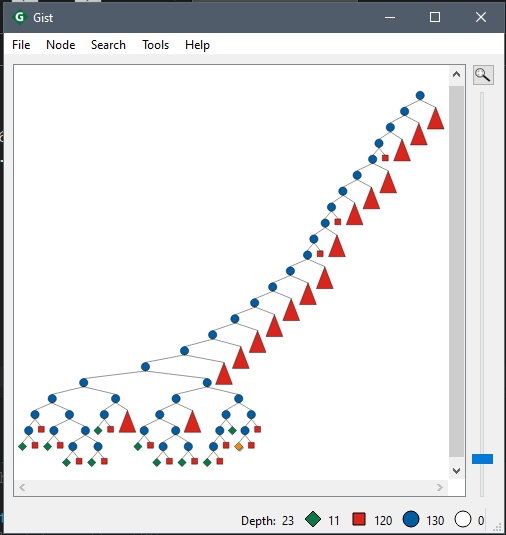
\includegraphics[width=0.5\textwidth]{Prueba1.png}
\caption{Árbol de decisión - prueba número 1}
\end{figure}

\vspace{0.5cm}

\begin{figure}[H]
\centering
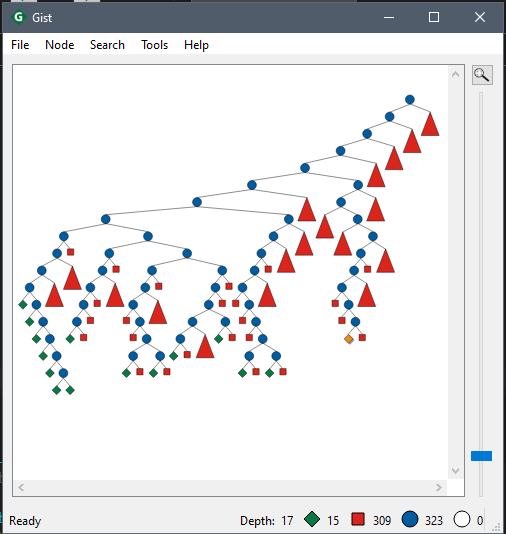
\includegraphics[width=0.5\textwidth]{Prueba2.png}
\caption{Árbol de decisión - prueba número 2}
\end{figure}

\newpage

\section{Instancias y pruebas}

\subsection{Instancias de prueba provistas}

Se nos asignó una batería de pruebas compuesta por 30 instancias. En todos los casos se logró encontrar soluciones óptimas. Para la ejecución del modelo, se utilizó el solver HiGHS a través de la biblioteca MiniZinc integrada en Python. En la tabla que se presenta a continuación, se pueden observar los resultados obtenidos para algunas de estas pruebas.

\begin{table}[H]
	\centering
	\caption{Resumen de resultados - Pruebas provistas}
	\rowcolors{2}{gray!20}{white}
	\begin{tabular}{|c|c|c|c|c|c|c|c|}
		\hline
		\rowcolor{gray!30}
		\textbf{Prueba} & \textbf{Costo} & \textbf{Soluciones} & \textbf{Tiempo} & \textbf{Nodos} & \textbf{Fallos} & \textbf{Valor Óptimo} \\
		\hline
		0   &  6.3 & 16   & 562ms  & 649   & 309   & 6.3 \\
		2     & 4.582  &  11 & 0.019ms  &  235 & 107  & 4.582 \\
		3   &  0.261 &  12  & 0.101ms &  163  &   69   & 0.261 \\
		4   & 1.06 & 38  & 118ms  & 1738 & 831  & 1.06 \\
		6  & 9.583 & 8 &  288ms  &  4876 &  2430  & 9.583   \\
		\hline
	\end{tabular}
\end{table}

\subsection{Instancias adicionales generadas}

Creamos un conjunto de 5 instancias personalizadas, cuyos resultados se detallan a continuación:

\begin{table}[H]
	\centering
	\caption{Resumen de resultados - Pruebas generadas}
	\rowcolors{2}{gray!20}{white}
	\begin{tabular}{|c|c|c|c|c|c|c|c|}
		\hline
		\rowcolor{gray!30}
		\textbf{Prueba} & \textbf{Costo} & \textbf{Soluciones} & \textbf{Tiempo} & \textbf{Nodos} & \textbf{Fallos} & \textbf{Valor Óptimo} \\
		\hline
		1   &  11.9 & 13   & 10.39s  & 250981   & 125478   & 17.38 \\
		2     & 35.0  &  6 & 390ms  &  109 & 49  & 5.3 \\
		3   &  55.6 &  21  & 2.3ms &  107  & 0 & 12.326 \\
		4   & 145 & 35  & 11.08ms  & 163,369 & 81,650  & 9.7 \\
		5  & 16.9985 & 15 & 1.78s  & 35883 &  17927  & 13.521 \\
		\hline
	\end{tabular}
\end{table}

Las instancias utilizadas son adecuadas para evaluar el modelo, ya que presentan una variedad de condiciones que permiten analizar su desempeño de forma integral. Se incluye diversidad en tamaños y extremismos ($p$ y $e$), lo cual permite observar cómo el modelo responde ante elementos con demandas muy distintas. Además, se emplean matrices de costos ($c$) no uniformes, es decir, estructuras en las que los valores de transporte entre elementos varían significativamente en lugar de mantenerse constantes o simétricos. Esto obliga al modelo a buscar rutas realmente eficientes en lugar de elegir caminos evidentes o arbitrarios.

Asimismo, las restricciones impuestas ($ct$ y $M$) fueron definidas para evitar soluciones triviales, exigiendo que el modelo realice un proceso de optimización más riguroso. Finalmente, al mantener constante el número de elementos y variar otros parámetros, se facilita el análisis del impacto que generan pequeños cambios en los datos sobre la solución final.

\section{Análisis de resultados}

A partir de las instancias tanto provistas como generadas, se observa que el modelo implementado en MiniZinc y ejecutado mediante Python ofrece una solución robusta y eficiente. Para las $30$ pruebas provistas, el modelo fue capaz de encontrar soluciones óptimas en todos los casos. Las métricas reportadas muestran tiempos de ejecución razonables, incluso en pruebas con múltiples soluciones factibles y árboles de decisión más complejos. Por ejemplo, la prueba $0$ entregó $16$ soluciones factibles en menos de $600 \text{ms}$, mientras que la prueba $4$ alcanzó $38$ soluciones factibles con más de $1,700$ nodos explorados, demostrando eficiencia y consistencia.

En cuanto a las instancias adicionales generadas por el equipo, estas fueron diseñadas para desafiar la capacidad de adaptación del modelo a condiciones más exigentes. Algunas instancias, como la prueba $1$ generada, requirieron más de $10$ segundos de cómputo y recorrieron más de $250,000$ nodos, reflejando una complejidad elevada. Sin embargo, se lograron soluciones satisfactorias en todos los casos, validando la capacidad del modelo para responder a diversas condiciones iniciales, restricciones ajustadas y estructuras de costos no uniformes.

\section{Conclusiones}

El proyecto logró cumplir con todos los objetivos propuestos: diseñar un modelo matemático que permita minimizar el extremismo en una población, formularlo en MiniZinc, resolverlo con métodos exactos (como Branch and Bound) y analizar la eficiencia del enfoque propuesto.

Los resultados muestran que el modelo es capaz de encontrar soluciones óptimas en tiempo razonable para instancias pequeñas y medianas. Además, el uso de estructuras de costos complejas y restricciones no triviales permitió validar su aplicabilidad en escenarios reales.

El análisis del algoritmo Branch and Bound muestra su capacidad de reducir el espacio de búsqueda mediante poda efectiva, lo que lo hace útil para problemas combinatorios con restricciones.

Entre las ventajas del enfoque propuesto se destacan:

\begin{itemize}
	\item La expresividad del modelo y su capacidad de adaptación a nuevas condiciones.

	\item La facilidad de integración con Python para gestionar instancias y automatizar pruebas.

	\item La representación clara de los árboles de decisión para entender el comportamiento del algoritmo.
\end{itemize}

Sin embargo, también se identifican limitaciones en escalabilidad, dado que para instancias muy grandes el tiempo de ejecución puede volverse excesivo.

En resumen, se implementó un modelo exacto, eficiente y adaptable, que logra minimizar el extremismo de opiniones bajo condiciones realistas. Este trabajo sienta las bases para futuras extensiones, como modelos más dinámicos o versiones heurísticas que ofrezcan soluciones más rápidas en contextos de gran escala.

\end{document}
